\hypertarget{Digital Twin Implementation}{%
\section{Digital Twin Implementation}\label{Digital Twin Implementation}}

Traditionally, automotive industry has long practiced the gradual transition from virtual, to hybrid, to physical phases within an X-in-the-loop (XIL; X = model, software, processor, hardware, vehicle) framework. Furthermore, recent modeling \& simulation methodologies such as simulation-as-a-service (SAAS) complemented with simulation-to-reality (sim2real) transfer show promise in facilitating parallelized scenario-based validation to enable robust system development and comprehensive corner-case analysis. However, the lack of physically realistic simulation of perception characteristics, system dynamics and agent-environment interactions, along with associated uncertainties, restricts the scalability and reliability of simulation-based verification. 

In such a milieu, digital twins have emerged as potentially viable tools to improve simulation fidelity and to develop adaption/augmentation techniques that can help bridge the sim2real gap. The following sections delve into the development of physically and graphically accurate vehicle and environment digital twins, and also discuss the integration of these with APIs and HMIs for developing autonomy-oriented applications.

\hypertarget{Vehicle Digital Twins}{%
\subsection{Vehicle Digital Twins}\label{Vehicle Digital Twins}}

\begin{figure}[t]
    \centering
    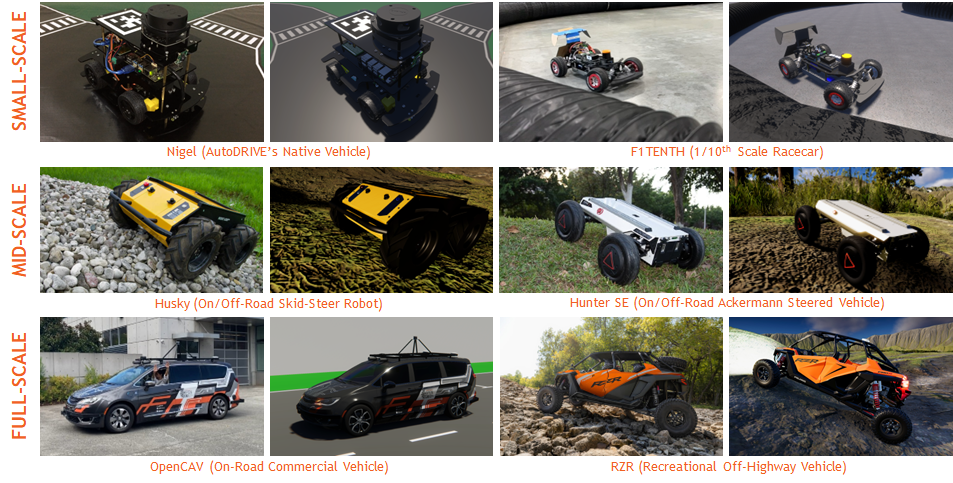
\includegraphics[width=\linewidth]{Figures/fig4.png}
    \caption{Autonomy-oriented vehicle digital twins across scales: Nigel and F1TENTH (small-scale), Husky and Hunter SE (mid-scale), and OpenCAV and RZR (full-scale) platforms for on/off-road autonomy.}
    \label{fig: figure4}
\end{figure}

As described earlier, we leveraged AutoDRIVE Simulator \cite{AutoDRIVESimulator, AutoDRIVESimulatorReport} to develop digital twin models of six different vehicles, across different scales and ODDs (Fig. \ref{fig: figure4}). These included small-scale (Nigel and F1TENTH), mid-scale (Husky and Hunter SE) and full-scale (OpenCAV and RZR) vehicles targeted towards on-road as well as off-road autonomy. It is to be noted that Husky and RZR fall purely under off-road ODD, and since this project (as well as Autoware) primarily targets on-road autonomy, these platforms have not been discussed elaborately in this report. Additionally, since this course focused on ``scaled autonomous vehicles'', the following sections describe Nigel and F1TENTH digital twins in detail; mid-scale (Hunter SE) and full-scale (OpenCAV) vehicle digital twins were outside the scope of this project (refer Section \ref{Work Breakdown Structure}), and as such the details pertaining to these have been discussed in limited scope.

From a computational perspective, the said simulation framework was developed modularly using object-oriented programming (OOP) constructs. Additionally, the simulator took advantage of CPU multi-threading as well as GPU instancing (if available) to efficiently handle the workload, while providing cross-platform support.

\subsubsection{Vehicle Dynamics Models}
\label{Sub-Section: Vehicle Dynamics Models}

The vehicle model is a combination of a rigid body and a collection of sprung masses $^iM$, where the total mass of the rigid body is defined as $M=\sum{^iM}$. The rigid body's center of mass, $X_{COM} = \frac{\sum{{^iM}*{^iX}}}{\sum{^iM}}$, connects these representations, with $^iX$ representing the coordinates of the sprung masses.

\begin{figure}[h]
     \centering
     \begin{subfigure}[b]{0.49\linewidth}
         \centering
         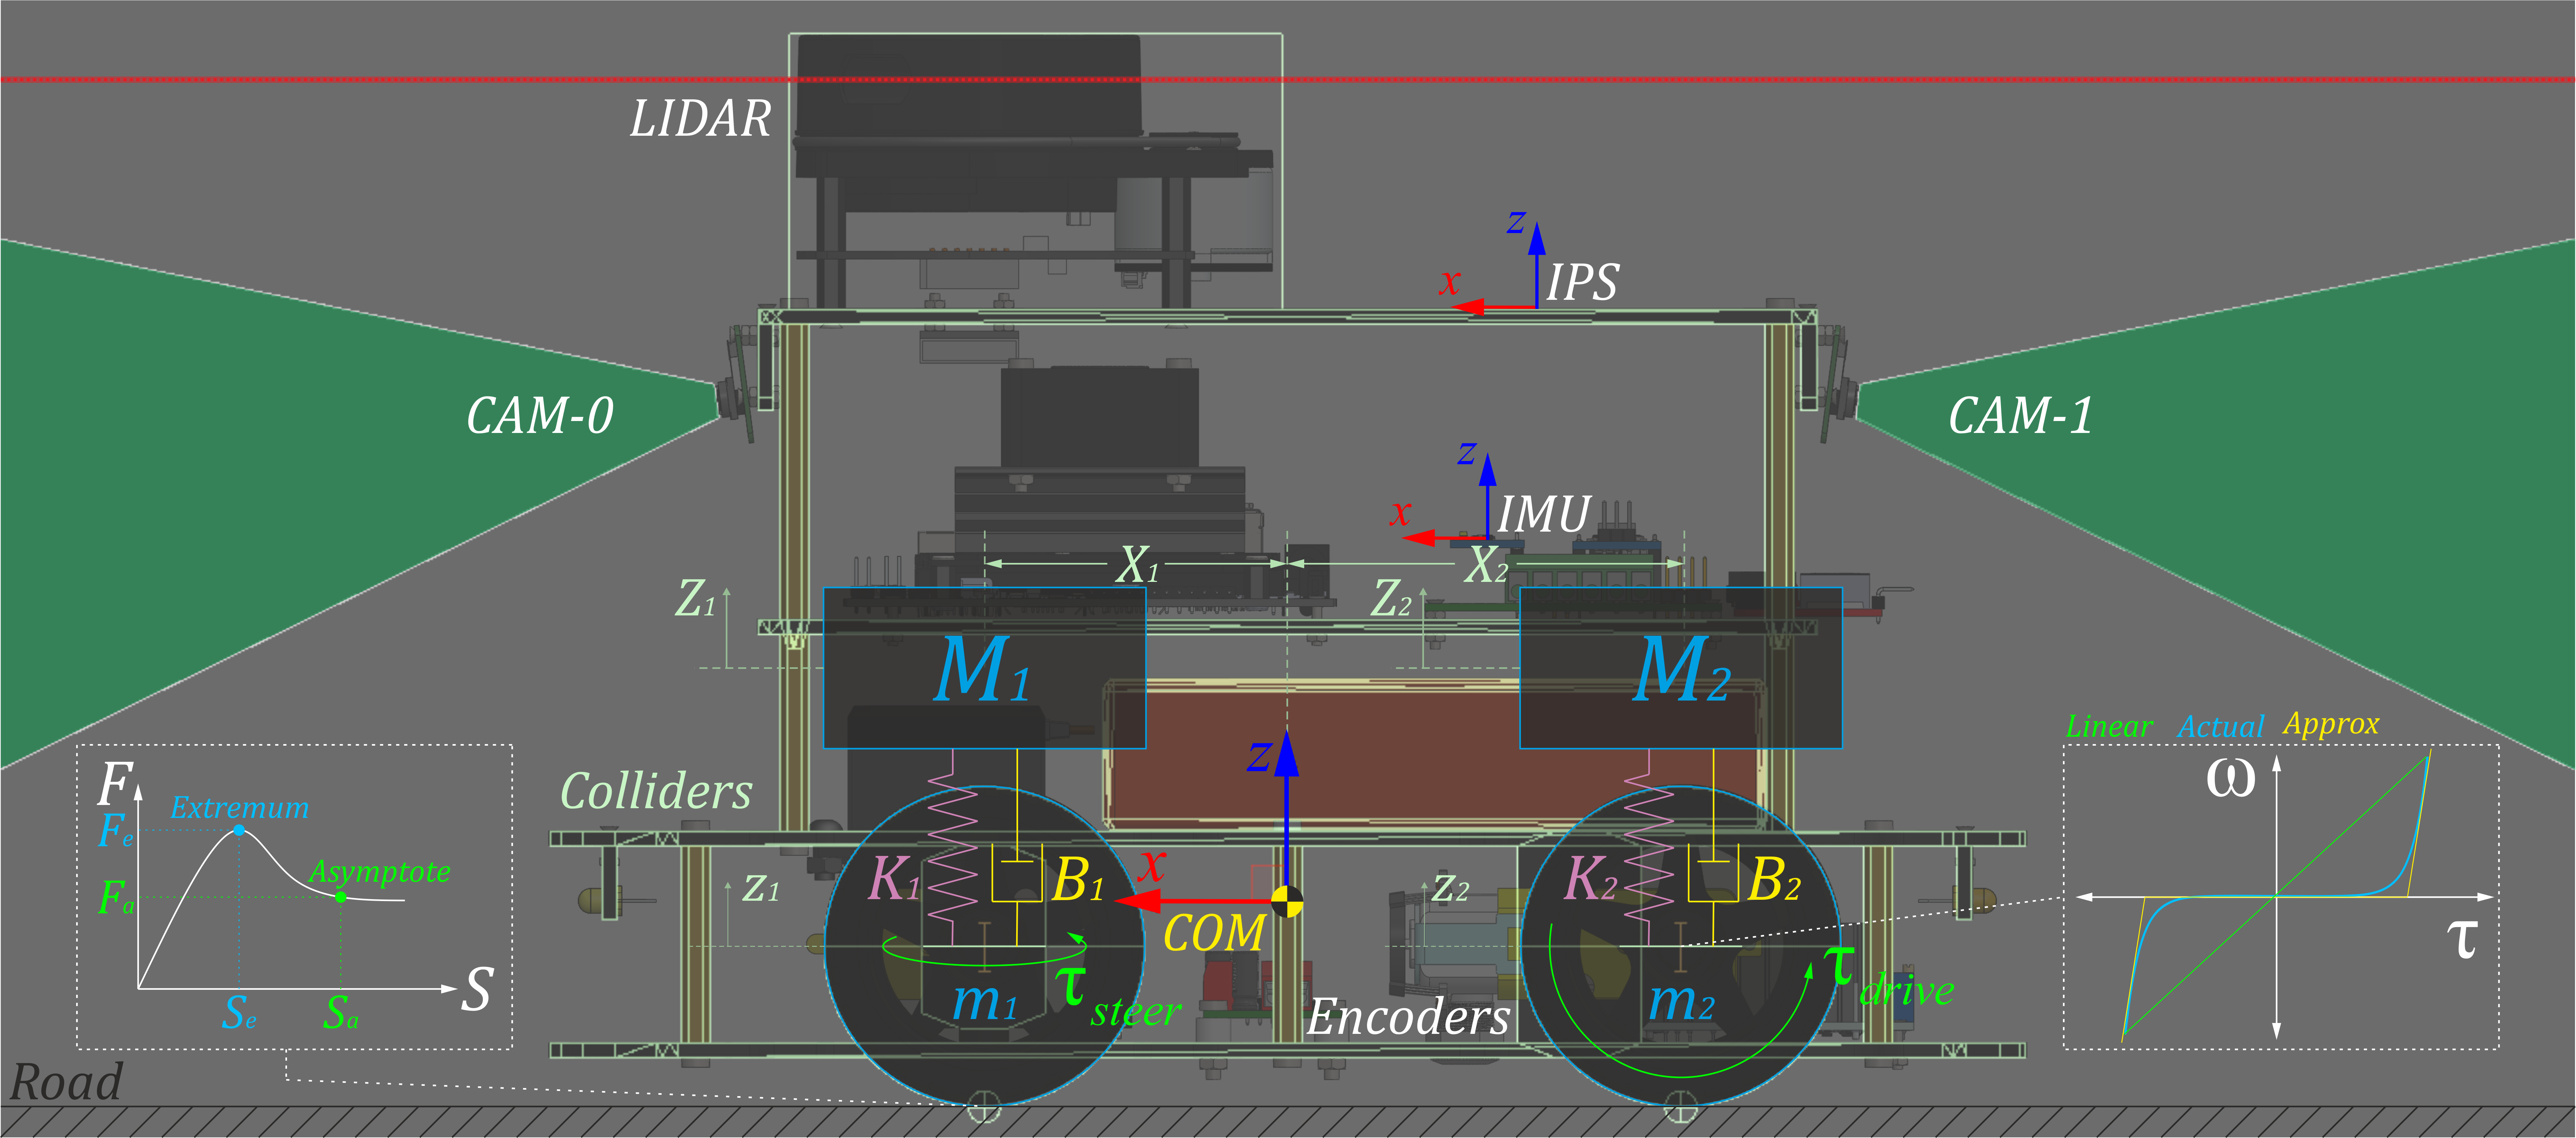
\includegraphics[width=\linewidth]{Fig5a.png}
         \caption{Nigel}
         \label{fig5a}
     \end{subfigure}
     \hfill
     \begin{subfigure}[b]{0.49\linewidth}
         \centering
         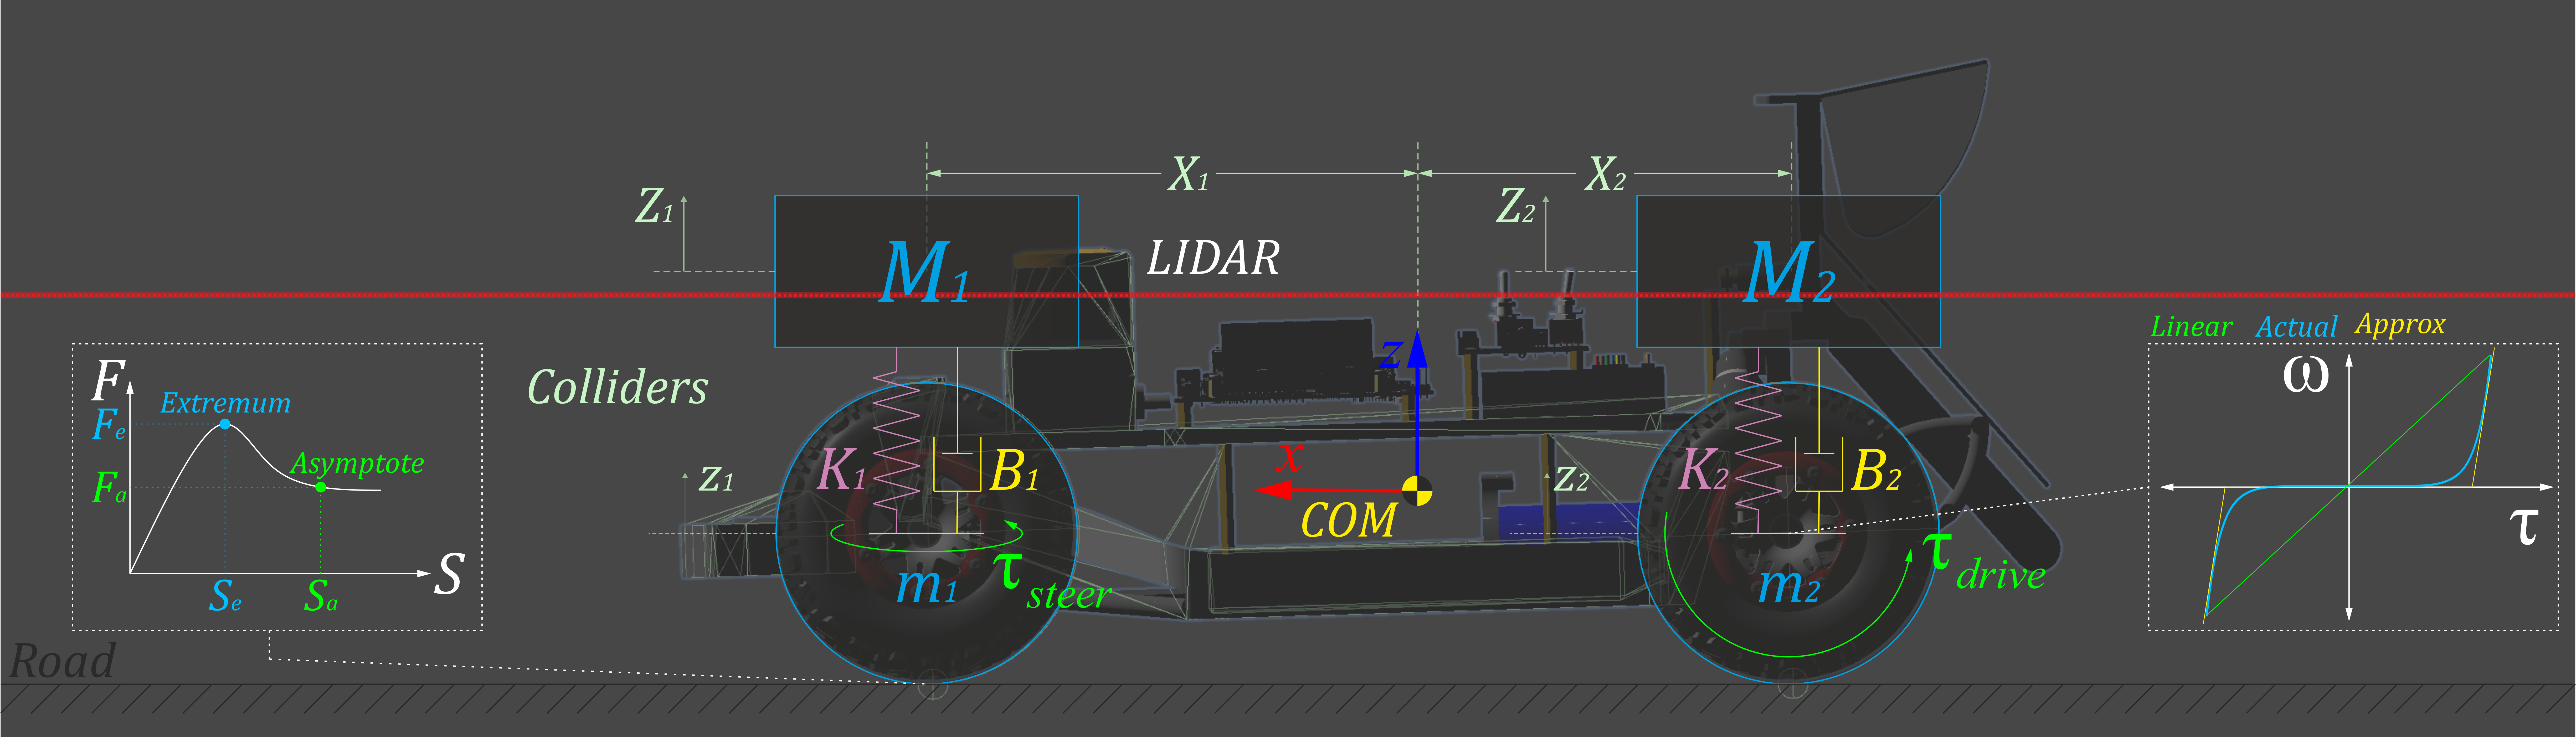
\includegraphics[width=\linewidth]{Fig5b.png}
         \caption{F1TENTH}
         \label{fig5b}
     \end{subfigure}
     \caption{Simulation of vehicle dynamics, sensors and actuators for Nigel and F1TENTH digital twins.}
    \label{figure5}
\end{figure}

The suspension force acting on each sprung mass is computed as ${^iM} * {^i{\ddot{Z}}} + {^iB} * ({^i{\dot{Z}}}-{^i{\dot{z}}}) + {^iK} * ({^i{Z}}-{^i{z}})$, where $^iZ$ and $^iz$ are the displacements of sprung and unsprung masses, and $^iB$ and $^iK$ are the damping and spring coefficients of the $i$-th suspension, respectively.

The vehicle's wheels are also treated as rigid bodies with mass $m$, subject to gravitational and suspension forces: ${^im} * {^i{\ddot{z}}} + {^iB} * ({^i{\dot{z}}}-{^i{\dot{Z}}}) + {^iK} * ({^i{z}}-{^i{Z}})$.

\sloppy Tire forces are computed based on the friction curve for each tire, represented as $\left\{\begin{matrix} {^iF_{t_x}} = F(^iS_x) \\{^iF_{t_y}} = F(^iS_y) \\ \end{matrix}\right.$, where $^iS_x$ and $^iS_y$ are the longitudinal and lateral slips of the $i$-th tire, respectively. The friction curve is approximated using a two-piece cubic spline, defined as $F(S) = \left\{\begin{matrix} f_0(S); \;\; S_0 \leq S < S_e \\ f_1(S); \;\; S_e \leq S < S_a \\ \end{matrix}\right.$, where $f_k(S) = a_k*S^3+b_k*S^2+c_k*S+d_k$ is a cubic polynomial function. The first segment of the spline ranges from zero $(S_0,F_0)$ to an extremum point $(S_e,F_e)$, while the second segment ranges from the extremum point $(S_e, F_e)$ to an asymptote point $(S_a, F_a)$.

The tire slip is influenced by factors including tire stiffness $^iC_\alpha$, steering angle $\delta$, wheel speeds $^i\omega$, suspension forces $^iF_s$, and rigid-body momentum $^iP$. These factors impact the longitudinal and lateral components of the vehicle's linear velocity. The longitudinal slip $^iS_x$ of the $i$-th tire is calculated by comparing the longitudinal components of the surface velocity of the $i$-th wheel (i.e., longitudinal linear velocity of the vehicle) $v_x$ with the angular velocity $^i\omega$ of the $i$-th wheel: ${^iS_x} = \frac{{^ir}*{^i\omega}-v_x}{v_x}$. The lateral slip $^iS_y$ depends on the tire's slip angle $\alpha$ and is determined by comparing the longitudinal $v_x$ (forward velocity) and lateral $v_y$ (side-slip velocity) components of the vehicle's linear velocity: ${^iS_y} = \tan(\alpha) = \frac{v_y}{\left| v_x \right|}$.

\subsubsection{Sensor Models}
\label{Sub-Section: Sensor Models}

The simulated vehicles can be equipped with the physically accurate interoceptive as well as exteroceptive sensing modalities. Specifically, the throttle ($\tau$) and steering ($\delta$) sensors are simulated using a straightforward feedback loop.

Incremental encoders are simulated by measuring the rotation of the rear wheels (i.e., the output shaft of driving actuators): $^iN_{ticks} = {^iPPR} * {^iGR} * {^iN_{rev}}$, where $^iN_{ticks}$ represents the ticks measured by the $i$-th encoder, $^iPPR$ is the base resolution (pulses per revolution) of the $i$-th encoder, $^iGR$ is the gear ratio of the $i$-th motor, and $^iN_{rev}$ represents the number of revolutions of the output shaft of the $i$-th motor.

The Inertial Positioning System (IPS) and Inertial Measurement Unit (IMU) are simulated based on temporally-coherent rigid-body transform updates of the vehicle $\{v\}$ with respect to the world $\{w\}$: ${^w\mathbf{T}_v} = \left[\begin{array}{c | c} \mathbf{R}_{3 \times 3} & \mathbf{t}_{3 \times 1} \\ \hline \mathbf{0}_{1 \times 3} & 1 \end{array}\right] \in SE(3)$. The IPS provides 3-DOF positional coordinates $\{x,y,z\}$ of the vehicle, while the IMU supplies linear accelerations $\{a_x,a_y,a_z\}$, angular velocities $\{\omega_x,\omega_y,\omega_z\}$, and 3-DOF orientation data for the vehicle, either as Euler angles $\{\phi_x,\theta_y,\psi_z\}$ or as a quaternion $\{q_0,q_1,q_2,q_3\}$.

The LIDAR simulation employs iterative ray-casting \texttt{raycast}\{$^w\mathbf{T}_l$, $\vec{\mathbf{R}}$, $r_{max}$\} for each angle $\theta \in \left [ \theta_{min}:\theta_{res}:\theta_{max} \right ]$ at an approximate update rate of 7 Hz. Here, ${^w\mathbf{T}_l} = {^w\mathbf{T}_v} * {^v\mathbf{T}_l} \in SE(3)$ represents the relative transformation of the LIDAR \{$l$\} with respect to the vehicle \{$v$\} and the world \{$w$\}, $\vec{\mathbf{R}} = \left [r_{max}*sin(\theta) \;\; r_{min}*cos(\theta) \;\; 0 \right ]^T$ defines the direction vector of each ray-cast $R$, where $r_{min}=$ 0.15 m and $r_{max}=$ 12 m denote the minimum and maximum linear ranges of the LIDAR, $\theta_{min}=0^\circ$ and $\theta_{max}=360^\circ$ set the minimum and maximum angular ranges of the LIDAR, and $\theta_{res}=1^\circ$ represents the angular resolution of the LIDAR. The laser scan ranges are determined by checking ray-cast hits and then applying a threshold to the minimum linear range of the LIDAR, calculated as \texttt{ranges[i]}$=\begin{cases} \texttt{hit.dist} & \text{ if } \texttt{ray[i].hit} \text{ and } \texttt{hit.dist} \geq r_{min} \\ \infty & \text{ otherwise} \end{cases}$, where \texttt{ray.hit} is a Boolean flag indicating whether a ray-cast hits any colliders in the scene, and \texttt{hit.dist}$=\sqrt{(x_{hit}-x_{ray})^2 + (y_{hit}-y_{ray})^2 + (z_{hit}-z_{ray})^2}$ calculates the Euclidean distance from the ray-cast source $\{x_{ray}, y_{ray}, z_{ray}\}$ to the hit point $\{x_{hit}, y_{hit}, z_{hit}\}$.

The simulated physical cameras are parameterized by their focal length ($f=$ 3.04 mm), sensor size ($\{s_x, s_y\} = $ \{3.68, 2.76\} mm), target resolution (default = 720p), as well as the distances to the near and far clipping planes ($N=$ 0.01 m and $F=$ 1000 m). The viewport rendering pipeline for the simulated cameras operates in three stages. First, the camera view matrix $\mathbf{V} \in SE(3)$ is computed by obtaining the relative homogeneous transform of the camera $\{c\}$ with respect to the world $\{w\}$: $\mathbf{V} = \begin{bmatrix} r_{00} & r_{01} & r_{02} & t_{0} \\ r_{10} & r_{11} & r_{12} & t_{1} \\ r_{20} & r_{21} & r_{22} & t_{2} \\ 0 & 0 & 0 & 1 \\ \end{bmatrix}$, where $r_{ij}$ and $t_i$ denote the rotational and translational components, respectively. Next, the camera projection matrix $\mathbf{P} \in \mathbb{R}^{4 \times 4}$ is calculated to project world coordinates into image space coordinates: $\mathbf{P} = \begin{bmatrix} \frac{2*N}{R-L} & 0 & \frac{R+L}{R-L} & 0 \\ 0 & \frac{2*N}{T-B} & \frac{T+B}{T-B} & 0 \\ 0 & 0 & -\frac{F+N}{F-N} & -\frac{2*F*N}{F-N} \\ 0 & 0 & -1 & 0 \\ \end{bmatrix}$, where $N$ and $F$ represent the distances to the near and far clipping planes of the camera, and $L$, $R$, $T$, and $B$ denote the left, right, top, and bottom offsets of the sensor. The camera parameters $\{f,s_x,s_y\}$ are related to the terms of the projection matrix as follows: $f = \frac{2*N}{R-L}$, $a = \frac{s_y}{s_x}$, and $\frac{f}{a} = \frac{2*N}{T-B}$. The perspective projection from the simulated camera's viewport is given as $\mathbf{C} = \mathbf{P}*\mathbf{V}*\mathbf{W}$, where $\mathbf{C} = \left [x_c\;\;y_c\;\;z_c\;\;w_c \right ]^T$ represents image space coordinates, and $\mathbf{W} = \left [x_w\;\;y_w\;\;z_w\;\;w_w \right ]^T$ represents world coordinates. Finally, this camera projection is transformed into normalized device coordinates (NDC) by performing perspective division (i.e., dividing throughout by $w_c$), leading to a viewport projection achieved by scaling and shifting the result and then utilizing the rasterization process of the graphics API (e.g., DirectX for Windows, Metal for macOS, and Vulkan for Linux). Additionally, a post-processing step simulates lens and film effects, such as lens distortion, depth of field, exposure, ambient occlusion, contact shadows, bloom, motion blur, film grain, chromatic aberration, etc.

\subsubsection{Actuator Models}
\label{Sub-Section: Actuator Models}

The vehicle's motion is controlled by driving and steering actuators, with response delays and saturation limits matched to their real-world counterparts by tuning their torque profiles and actuation limits.

The driving actuators propel the rear/front/all wheels by applying a torque, calculated as ${^i\tau_{drive}} = {^iI_w}*{^i\dot{\omega}_w}$, where ${^iI_w} = \frac{1}{2}*{^im_w}*{^i{r_w}^2}$ represents the moment of inertia, $^i\dot{\omega}_w$ is the angular acceleration, $^im_w$ is the mass, and $^ir_w$ is the radius of the $i$-th wheel. Additionally, the driving actuators simulate holding torque by applying an idle motor torque equivalent to the braking torque, i.e., ${^i\tau_{idle}} = {^i\tau_{brake}}$.

The front wheels are steered using a steering actuator that generates a torque proportional to the required angular acceleration, given by $\tau_{steer} = I_{steer}*\dot{\omega}_{steer}$. The individual turning angles, $\delta_l$ and $\delta_r$, for the left and right wheels, respectively, are computed based on the commanded steering angle $\delta$, utilizing the Ackermann steering geometry defined by the wheelbase $l$ and track width $w$, as follows: $\left\{\begin{matrix} \delta_l = \textup{tan}^{-1}\left(\frac{2*l*\textup{tan}(\delta)}{2*l+w*\textup{tan}(\delta)}\right) \\ \delta_r = \textup{tan}^{-1}\left(\frac{2*l*\textup{tan}(\delta)}{2*l-w*\textup{tan}(\delta)}\right) \end{matrix}\right.$

\subsubsection{Calibration and Validation}
\label{Sub-Section: Calibration and Validation}

The vehicle digital twin models were calibrated and validated against geometric, static and dynamic measurement data collected from their real-world counterparts and/or their datasheets. This included the validation of geometric measurements for physical as well as visual purposes, static calibration for mass and center of mass parameters and dynamic calibration for validating standard benchmark maneuvers performed in open-loop tests. Additionally, sensor models were validated against static and dynamic characteristics of their real-world counterparts. Fig. \ref{fig: figure6} depicts some of these calibration/validation tests.

\begin{figure}[t]
    \centering
    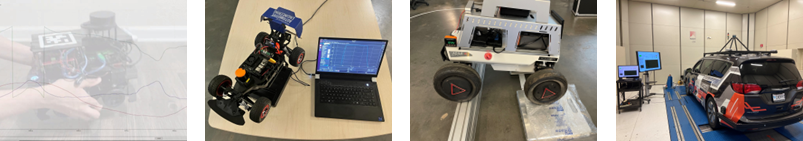
\includegraphics[width=\linewidth]{Figures/fig6.png}
    \caption{Calibration and validation of vehicle digital twins: IMU calibration/validation of Nigel, VESC calibration/validation of F1TENTH, static measurements of Hunter SE, and powertrain measurements of OpenCAV.}
    \label{fig: figure6}
\end{figure}

\subsubsection{Physical Vehicle Build and Setup}
\label{Sub-Section: Physical Vehicle Build and Setup}

We predominantly worked with two small-scale physical vehicles during the course of this project. These included an F1TENTH and a Nigel. While the prior was acquired off-the-shelf, its hardware and software had to be tested, configured, calibrated and set up to interface with the \href{https://github.com/Tinker-Twins/AutoDRIVE-F1TENTH}{ROS}, \href{https://github.com/Tinker-Twins/AutoDRIVE-F1TENTH}{ROS 2} and \href{https://github.com/Tinker-Twins/AutoDRIVE-Autoware}{Autoware} stacks. The latter, on the other hand, was designed, manufactured and assembled from scratch, including its \href{https://github.com/AutoDRIVE-Ecosystem/Nigel-SolidWorks}{mechanical} and \href{https://github.com/AutoDRIVE-Ecosystem/Nigel-Fritzing}{electronic} subsystems, \href{https://github.com/AutoDRIVE-Ecosystem/Nigel-Arduino}{firmware development} as well as \href{https://github.com/Tinker-Twins/AutoDRIVE/tree/AutoDRIVE-Devkit/ADSS Toolkit/autodrive_ros/autodrive_nigel}{ROS}, \href{https://github.com/Tinker-Twins/AutoDRIVE/tree/AutoDRIVE-Devkit/ADSS Toolkit/autodrive_ros2/autodrive_nigel}{ROS 2} and \href{https://github.com/Tinker-Twins/AutoDRIVE-Autoware}{Autoware} integration.

\begin{figure}[h]
    \centering
    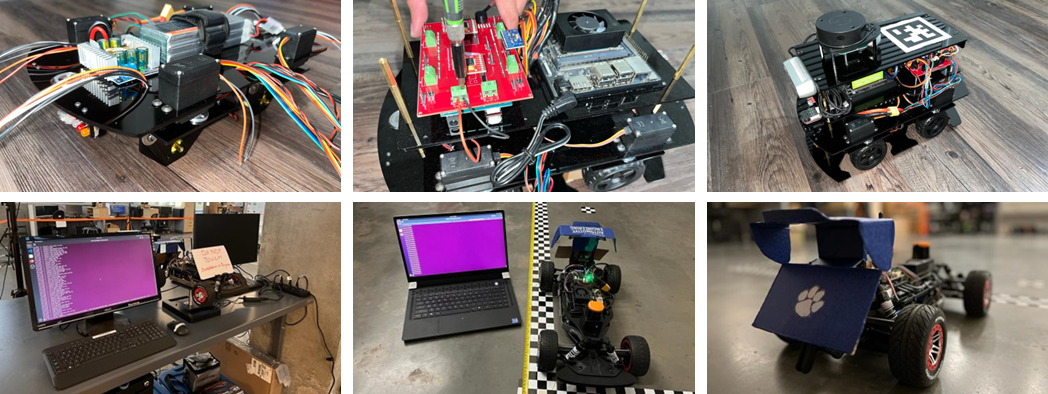
\includegraphics[width=\linewidth]{Figures/fig7.png}
    \caption{Physical build and setup depicting the progress stages during the hardware/software build, calibration and testing of F1TENTH and Nigel vehicles.}
    \label{fig: figure7}
\end{figure}

Being open-source vehicles, build documentation for \href{https://f1tenth.org/build.html}{F1TENTH} and \href{https://github.com/Tinker-Twins/AutoDRIVE/blob/AutoDRIVE-Testbed/Documents/Nigel - Assembly Guide.pdf}{Nigel} are readily available online. Fig. \ref{fig: figure7} depicts intermittent stages in building and setting up these vehicles.

\hypertarget{Environment Digital Twins}{%
\subsection{Environment Digital Twins}\label{Environment Digital Twins}}

\begin{figure}[h]
    \centering
    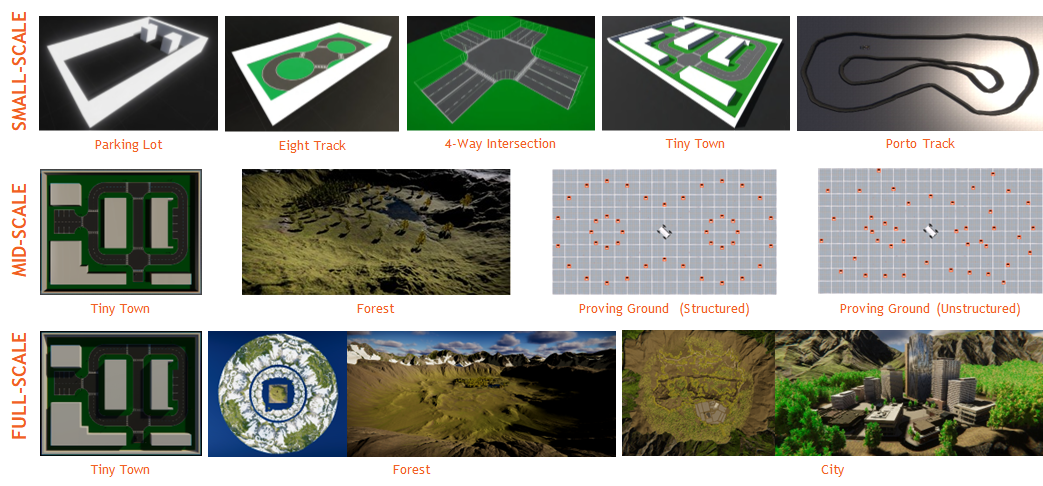
\includegraphics[width=\linewidth]{Figures/fig8.png}
    \caption{Autonomy-oriented environment digital twins across scales: Parking Lot, Eight Track, 4-Way Intersection, Tiny Town and Porto Track (small-scale), Tiny Town, Forest and Proving Ground (mid-scale), and Tiny Town, Forest and City (full-scale) scenarios for on/off-road autonomy.}
    \label{fig: figure8}
\end{figure}

As described earlier, we leveraged AutoDRIVE Simulator \cite{AutoDRIVESimulator, AutoDRIVESimulatorReport} to develop digital twin models of various environments, across different scales and ODDs (Fig. \ref{fig: figure8}). These included realistic counterparts of small-scale environments such as the Parking Lot, Eight Track, 4-Way Intersection and Tiny Town for Nigel, which were developed using AutoDRIVE IDK, as well as the Porto Track for F1TENTH, which was created based on the binary occupancy grid map of its real-world counterpart. Additionally, simplistic mid-scale and full-scale environments such as the scaled-up versions of Tiny Town along with structured and unstructured Proving Ground scenarios were developed. Finally, two highly detailed, albeit imaginary, mid-scale and full-scale scenarios were developed to support on-road as well as off-road autonomy. These included a City scenario and a Forest environment (Fig. \ref{figure9}). The full-scale variants of these scenarios have several rich features and are large enough to support driving for several minutes, if not a few hours. Additionally, these scenarios allowed the simulation of various environmental conditions, such as different times of day as well as weather conditions, to introduce additional degrees of variability. Finally, environmental physics was simulated accurately by conducting mesh-mesh interference detection and computing contact forces, frictional forces, momentum transfer, as well as linear and angular drag acting on all rigid bodies, at each time step.

\begin{figure}[h]
     \centering
     \begin{subfigure}[b]{0.49\linewidth}
         \centering
         \includegraphics[width=\linewidth]{Fig9a.png}
         \caption{City}
         \label{fig9a}
     \end{subfigure}
     \hfill
     \begin{subfigure}[b]{0.49\linewidth}
         \centering
         \includegraphics[width=\linewidth]{Fig9b.png}
         \caption{Forest}
         \label{fig9b}
     \end{subfigure}
     \caption{City and Forest environment digital twins depicting their respective highlights and features to support on-road as well as off-road autonomy.}
    \label{figure9}
\end{figure}

From a computational perspective, the said environment digital twins, especially the full-scale scenarios, made use of pre-baked lightmaps, which provided the benefits of physics-based lighting while reducing the computational overhead of real-time raytracing. Additionally, the simulator implemented level-of-detail (LOD) culling to gradually degrade the LOD of environmental objects as they moved further away from the scene cameras. However, it was ensured that LOD culling did not affect any of the AV camera sensor(s).

AutoDRIVE Simulator supports various approaches to developing realistic/imaginary environment digital twins:
\begin{itemize}
     \item \textit{AutoDRIVE IDK:} Custom scenarios and maps can be crafted by utilizing the modular and adaptable Infrastructure Development Kit (IDK). This kit provides the flexibility to configure terrain modules, road networks, obstruction modules, and traffic elements. Specifically, the Parking Lot, Eight Track, 4-Way Intersection, Tiny Town and Proving Ground scenarios were developed using AutoDRIVE IDK.

     \item \textit{Plug-In Scenarios:} AutoDRIVE Simulator supports third-party tools, such as RoadRunner \cite{RoadRunner}, and open standards like OpenSCENARIO \cite{OpenSCENARIO} and OpenDRIVE \cite{OpenDRIVE}). This allows users to incorporate a diverse range of plugins, packages, and assets in several standard formats for creating or customizing driving scenarios. Particularly, the autonomous racing scenario was created based on the binary occupancy grid map of a real-world F1TENTH racetrack called ``Porto'' using a third-party 3D modeling software, which was then imported into AutoDRIVE Simulator and post-processed with physical as well as graphical enhancements to make it ``sim-ready''.

     \item \textit{Unity Terrain Integration:} Since the AutoDRIVE Simulator is built atop the Unity \cite{Unity} game engine, it seamlessly supports scenario design and development through Unity Terrain \cite{UnityTerrain}. Users have the option to define terrain meshes, textures, heightmaps, vegetation, skyboxes, wind effects, and more, allowing the design of both on-road and off-road scenarios. This option is well-suited for modeling full-scale environments. Specifically, Forest and City scenes were developed using this technique.
\end{itemize}

\hypertarget{APIs and HMIs to Connect with Digital Twins}{%
\subsection{APIs and HMIs to Connect with Digital Twins}\label{APIs and HMIs to Connect with Digital Twins}}

\begin{figure}[h]
    \centering
    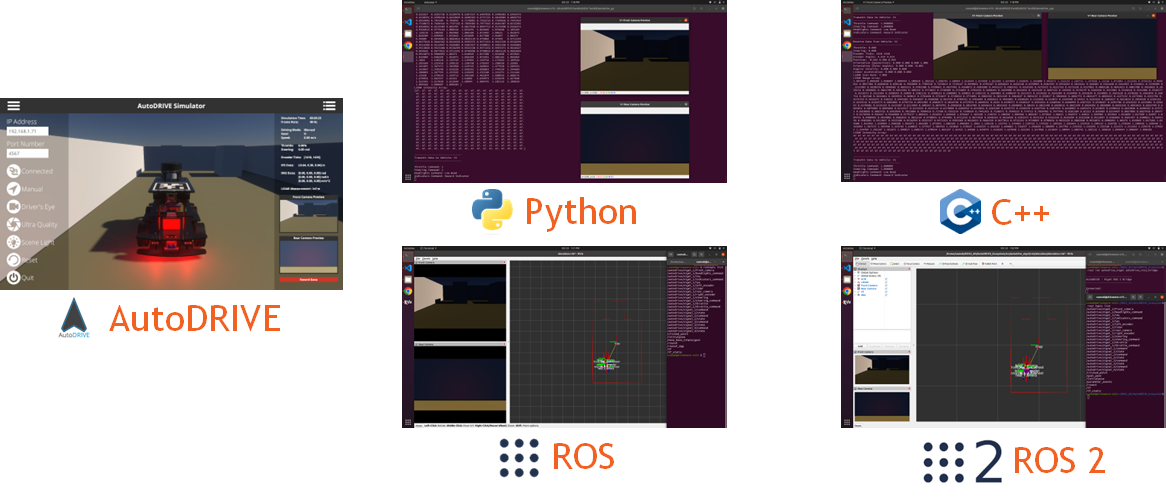
\includegraphics[width=\linewidth]{Figures/fig10.png}
    \caption{APIs to connect with AutoDRIVE Ecosystem: Python, C++, ROS and ROS 2. Note that AutoDRIVE-Autoware integration is accomplished by extending the ROS 2 API.}
    \label{fig: figure10}
\end{figure}

The integration of APIs within the AutoDRIVE Ecosystem was achieved through the comprehensive expansion and incorporation of AutoDRIVE Devkit. The versatile APIs developed as part of this framework facilitate interactions with the virtual/real vehicles using Python, C++, ROS, ROS 2, or the Autoware stack (Fig. \ref{fig: figure10}). This expansion caters to a diverse range of programming preferences, empowering users to exploit the AutoDRIVE Simulator or AutoDRIVE Testbed for swift and flexible development of autonomy algorithms. The framework extends its utility by enabling the development of API-mediated HMIs, catering to both virtual and physical vehicles.

\begin{figure}[t]
    \centering
    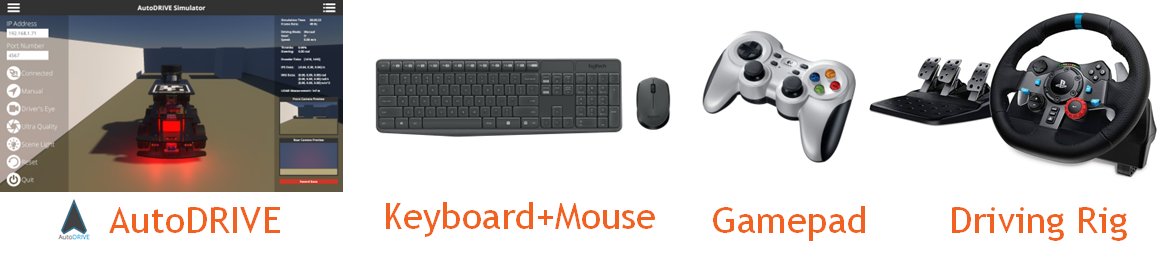
\includegraphics[width=\linewidth]{Figures/fig11.png}
    \caption{HMIs to connect with AutoDRIVE Ecosystem include standard keyboard (digital) and mouse (analog), gamepad/joystick (analog) as well as driving and steering rigs (hybrid).}
    \label{fig: figure11}
\end{figure}

Apart from the API-mediated HMIs, the simulation framework itself served a dual purpose by not only providing a digital twinning platform, but also enabling the development of direct HMIs to interface with the virtual vehicles (Fig. \ref{fig: figure11}). This direct-HMI teleoperation framework, designed for scalability, ensures practical feasibility by relaying identical machine-to-machine (M2M) commands to both virtual and real vehicles. The versatility of this approach allows for a true digital-twin framework, establishing a seamless connection between the simulated environment and the physical world. Additionally, in an extended-reality (XR) setup, this framework offers opportunities to extend the direct-HMI teleoperation to real vehicles, enhancing the applicability and potential of AutoDRIVE Ecosystem in diverse operational scenarios.